%
%===============>>  ГРУППА 9-2 МОДУЛЬ 7  <<=============
%
\setmodule{7}

%BEGIN_FOLD % ====>>_____ Занятие 1 _____<<====
\begin{class}[number=1]
	\begin{listofex}
		\item В треугольнике \( ABC \) угол \( C \) равен \( 90 \) градусов, \( AC=6 \), \( AB=20 \). Найдите \( \sin B \).
		\item  В треугольнике \( ABC \) угол \( C \) равен \( 90 \) градусов, \( BC=9 \), \( AB=20 \). Найдите \( \cos B \).
		\item В треугольнике \( ABC \) угол \( C \) равен \( 90 \) градусов, \( BC=9 \), \( AC=27 \). Найдите \( \tg B \).
		\item Найдите:
		\begin{tasks}(1)
			\task \( \sin\alpha \) и \( \tg\alpha \), если \( \cos\alpha=\dfrac{1}{2} \)
			\task \( \cos\alpha \) и \( \tg\alpha \), если \( \sin\alpha=\dfrac{\sqrt{3}}{2} \)
		\end{tasks}
		\item В треугольнике \( ABC \) угол \( C \) прямой, \( BC=8 \), \( \sin A=0,4 \). Найдите \( AB \).
		\item В треугольнике \( ABC \) угол \( C \) прямой, \( AC=15 \), \( \cos A=\dfrac{5}{7} \). Найдите \( AB \).
		\item В треугольнике \( ABC \) угол \( C \) равен \( 90\degree \), \( BC=12 \), \( \sin A=\dfrac{4}{11} \). Найдите \( AB \).
		\item Катеты прямоугольного треугольника равны \( \sqrt{15} \) и \( 1 \). Найдите синус наименьшего угла этого треугольника.
		\item Площадь прямоугольного треугольника равна \( 32\sqrt{3} \). Один из острых углов равен \( 30\degree \). Найдите длину гипотенузы.
		\item В треугольнике \( ABC \) угол \( C \) равен \( 90\degree \), \( AC=12 \), \( \tg A=\dfrac{2\sqrt{10}}{3} \).  Найдите \( AB \).
		\item В треугольнике \( ABC \) угол \( C \) равен \( 90\degree \), \( \sin A=\dfrac{4}{5} \), \( AC=9 \). Найдите \( AB \).
		\item Найдите синус меньшего острого угла между	диагональю прямоугольника и его стороной, если периметр прямоугольника равен \( 34 \) см, а одна из сторон --- \( 12 \) см. 
		\item Тангенс острого угла прямоугольного треугольника равен \( \dfrac{2}{5} \), а один из катетов на \( 6 \) см больше другого. Найдите площадь треугольника. 
		\item Основание равнобедренного треугольника равно \( 8 \) см, тангенс угла при основании равен \( 2 \). Найдите площадь треугольника. 
		\item Периметр равнобедренного треугольника равен \( 64 \) см, косинус угла при основании равен \( 0,6 \). Найдите площадь треугольника.
		\item В треугольнике \( ABC \) известно, что \( AB=8 \), \( BC=10 \), \( AC=12 \). Найдите \( \cos\angle ABC \).
		\item В треугольнике \( ABC \) сторона \( AB \) равна \( 2\sqrt{3} \), угол \( C \) равен \( 120\degree \). Найдите радиус описанной около этого треугольника окружности.
		\item Сторона правильного треугольника равна \( \sqrt{3} \). Найдите радиус окружности, описанной около этого треугольника.
		\item Найдите хорду, на которую опирается угол \( 120\degree \), вписанный в окружность радиуса \( \sqrt{3} \).  
		\item Сторона \( AB \) треугольника \( ABC \) равна \( 1 \). Противолежащий ей угол \( C \) равен \( 120\degree \). Найдите радиус окружности, описанной около этого треугольника.
		\item Угол \( C \) треугольника \( ABC \), вписанного в окружность радиуса \( 3 \), равен \( 30\degree \). Найдите сторону \( AB \) этого треугольника.
		\item Одна сторона остроугольного треугольника равна радиусу описанной около него окружности. Найдите угол треугольника, противолежащий этой стороне. Ответ дайте в градусах.
		\item В треугольнике \( ABC \) угол \( B \) равен \( 72\degree \), угол \( C \) равен \( 63\degree \), \( BC=2\sqrt{2} \). Найдите радиус описанной около этого треугольника окружности.
	\end{listofex}
\end{class}
%END_FOLD

%BEGIN_FOLD % ====>>_____ Занятие 2 _____<<====
\begin{class}[number=2]
	\begin{listofex}
		\item Выяснить вид треугольника (остроугольный, прямоугольный, тупоугольный), если длины его сторон равны \( 23 \) см, \( 17 \) см, \( 19 \) см. 
		\item Стороны треугольника равны \( 8\sqrt{3} \) см, \( \sqrt{577} \) см и \( \sqrt{11} \) см. Найдите наибольший угол	этого треугольника. 
		\item Две стороны параллелограмма равны \( 4 \) см и \( 5 \) см, а одна из диагоналей --- \( 46 \)
		см. Найти вторую диагональ параллелограмма.
		\item Боковая сторона равнобедренного треугольника равна \( 1 \), угол при вершине, противолежащей основанию, равен \( 120\degree \). Найдите диаметр описанной окружности этого треугольника.
		\item Радиус окружности, описанной около правильного треугольника, равен \( \sqrt{3} \). Найдите сторону этого треугольника.
		\item В треугольнике \( ABC \): \( \sin\angle B=0,6 \), \( AC=3 \), \( \angle C=30\degree \). Найдите \( AB \).
		\item Радиус окружности, описанной около треугольника \( ABC \), равен \( R \). Большая сторона треугольника \( ABC \) равна \( 10 \), а \( \angle ABC=150\degree \). Найдите \( R \).
		\item В треугольнике \( ABC \) проведена медиана \( AM \). Найдите площадь треугольника \( ABC \), если \( AC=3\sqrt{2} \), \( BC=10 \), \( \angle MAC=45\degree \).
		\item Площадь треугольника \( ABC \) равна \( 20\sqrt{3} \). Найдите \( AC \), если сторона \( AB \) равна \( 8 \), а медиана \( BM \) равна \( 5 \).
		\item В треугольнике \( ABC \): \( \angle A=45\degree \), \( O \) --- точка пересечения серединных перпендикуляров к сторонам \( AB \) и \( BC \), \( OD=44 \) --- серединный перпендикуляр к стороне \( CB \). Найдите \( CB \).
		\item Найдите угол \( ABC \), изображенный на рисунке. Ответ дайте в градусах.
		\begin{center}
			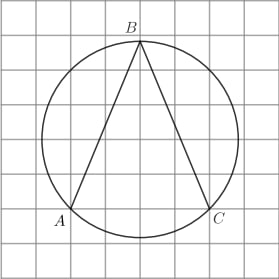
\includegraphics[align=t, width=0.3\linewidth]{\picpath/G92M7L2}
		\end{center}
		\item Найдите градусную меру дуги \( AC \) окружности, на которую опирается угол \( ABC \). Ответ
		дайте в градусах.
		\begin{center}
			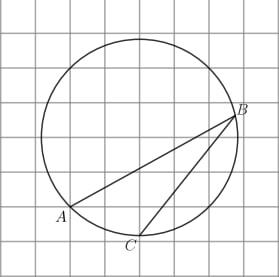
\includegraphics[align=t, width=0.3\linewidth]{\picpath/G92M7L2-2}
		\end{center}
		\item Найдите угол \( AOB \), изображенный на рисунке. Ответ дайте в градусах.
		\begin{center}
			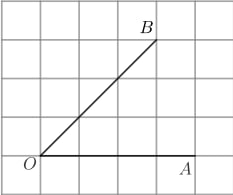
\includegraphics[align=t, width=0.3\linewidth]{\picpath/G92M7L2-3}
		\end{center}
		\item На клетчатой бумаге с размером клетки \( 1X1 \) изображён угол \( AOB \). Найдите его тангенс.
		\begin{center}
			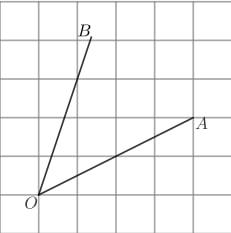
\includegraphics[align=t, width=0.3\linewidth]{\picpath/G92M7L2-4}
		\end{center}
	\end{listofex}
\end{class}
%END_FOLD

%BEGIN_FOLD % ====>>_ Домашняя работа 1 _<<====
\begin{homework}[number=1]
	\begin{listofex}
		\item В треугольнике \( ABC \) угол \( C \) равен \( 90\degree \), \( AC=9 \), \( AB=25 \). Найдите \( \sin B \).
		\item В треугольнике \( ABC \) угол \( C \) равен \( 90\degree \), BC\( =4 \), \( AC=28 \). Найдите \( \tg B \).
		\item В треугольнике \( ABC \) угол \( C \) равен \( 90\degree \), \( \sin B=\dfrac{5}{17} \), \( AB=51 \). Найдите \( AC \).
		\item В треугольнике\( ABC \) угол \( C \) равен \( 90\degree \), \( \tg B=\dfrac{8}{5} \), \( BC=20 \). Найдите \( AC \).
		\item Синус острого угла \( A \) треугольника \( ABC \) равен \( \dfrac{2\sqrt{6}}{5} \). Найдите \( \cos A \).
		\item В треугольнике \( ABC \) известно, что \( AB=6 \), \( BC=7 \), \( AC=8 \). Найдите \( \cos\angle ABC \).
		\item В треугольнике \( ABC \) угол \( A \) равен \( 60\degree \), угол \( B \) равен \( 45\degree \), \( BC=5\sqrt{6} \). Найдите \( AC \).
		\item Сторона правильного треугольника равна \( 3 \). Найдите радиус окружности, описанной около этого треугольника.
		\item В треугольнике \( ABC \) угол \( B \) равен \( 56\degree \), угол \( C \) равен \( 64\degree \), \( BC=3\sqrt{3} \). Найдите радиус описанной около этого треугольника окружности.
	\end{listofex}
\end{homework}
%END_FOLD

%BEGIN_FOLD % ====>>_____ Занятие 3 _____<<====
\begin{class}[number=3]
	\begin{listofex}
		\item Занятие 3 
	\end{listofex}
\end{class}
%END_FOLD

%BEGIN_FOLD % ====>>_____ Занятие 4 _____<<====
\begin{class}[number=4]
	\begin{listofex}
		\item Занятие 4
	\end{listofex}
\end{class}
%END_FOLD

%BEGIN_FOLD % ====>>_ Домашняя работа 2 _<<====
\begin{homework}[number=2]
	\begin{listofex}
		\item Домашняя работа 2
	\end{listofex}
\end{homework}
%END_FOLD

%BEGIN_FOLD % ====>>_____ Занятие 5 _____<<====
\begin{class}[number=5]
	\begin{listofex}
		\item Занятие 5
	\end{listofex}
\end{class}
%END_FOLD

%BEGIN_FOLD % ====>>_____ Занятие 6 _____<<====
\begin{class}[number=6]
	\begin{listofex}
		\item Занятие 6
	\end{listofex}
\end{class}
%END_FOLD

%BEGIN_FOLD % ====>>_ Домашняя работа 3 _<<====
\begin{homework}[number=3]
	\begin{listofex}
		\item Домашняя работа 3
	\end{listofex}
\end{homework}
%END_FOLD

%BEGIN_FOLD % ====>>_____ Занятие 7 _____<<====
\begin{class}[number=7]
	\title{Подготовка к проверочной}
	\begin{listofex}
		\item Занятие 7
	\end{listofex}
\end{class}
%END_FOLD

=%BEGIN_FOLD % ====>>_ Проверочная работа _<<====
\begin{exam}
	\begin{listofex}
		\item Проверочная
	\end{listofex}
\end{exam}
%END_FOLD